% ============================================================
% IE UNIVERSITY - BAM - ML & Communication Skills Project Proposal
% ============================================================

\documentclass[clean]{bam-proposal}
%\documentclass[annotated]{bam-proposal}

\BAMtitle{Early Collision Risk Forecasting from ESA Conjunction Data Messages}
\BAMteam{Pedro Jon Fuentes Garc\'es; Mario Fern\'andez Velasco}
\BAMcourse{Machine Learning \& Communication Skills}
\BAMacademicyear{2026--2027}
\BAMsubmissiondate{11 October 2026, 23:59 Madrid time}

\BAMbibliographystyle{plainnat}
\BAMbibliographyfile{references}

\begin{document}
\makeproposalheader

\section{Problem, Motivation, and Research Question}

Low Earth Orbit is increasingly congested. When two objects may approach closely, operators receive Conjunction Data Messages (CDMs) with geometry, covariance, and a self-computed collision risk. Over about one week before time of closest approach (TCA), several CDMs arrive; many events that look concerning early become clearly safe near TCA. Operators often begin avoidance planning about two days before TCA~\citep{kelvins2019challenge,uriot2021collision}.

\textbf{How this project differs from the ESA Kelvins competition.}
The 2019 Kelvins Collision Avoidance Challenge asked teams to minimise a single leaderboard loss \(L=\mathrm{MSE}_{\mathrm{HR}}/F_2\) on early CDMs~\citep{kelvins2019challenge,uriot2021collision}. We reuse that public dataset and the same early-input constraint (time-to-TCA \(\ge 2\) days), but our scientific goal is \emph{not} to climb that leaderboard or to reproduce winning competition pipelines. We treat Kelvins as a shared benchmark and prior art: we ask which modelling strategies improve upon a strong last-risk-prediction (LRP) baseline under rare-event metrics, with calibrated high-risk probabilities, explicit analysis of ``jump'' failures, and a transparent failure atlas. Success is decision-support insight and honest characterisation of uncertainty---not a competition ranking.

\textbf{Intended impact / outcome.}
If successful, the project delivers (i)~a reproducible event-level protocol comparing course and ambitious models against LRP under \(F_2\) and \(\mathrm{MSE}_{\mathrm{HR}}\); (ii)~evidence on whether a two-stage design---detect high risk, then estimate risk magnitude---better characterises uncertain near-TCA jumps than point estimates alone; and (iii)~an actionable failure atlas operators or analysts could use to know \emph{when not to trust} an early forecast. We do not claim operational deployment or autonomous commanding.

\textbf{Primary RQ.}
Given CDMs with time-to-TCA \(\ge 2\) days, which modelling approach best improves upon LRP for final collision risk under rare-event metrics \(F_2\) and \(\mathrm{MSE}_{\mathrm{HR}}\)?

\textbf{Secondary RQ.}
Can a calibrated high-risk probability in a two-stage design better characterise uncertain jump events---where risk rises sharply near TCA---than point estimates alone?

\textbf{Scope and ambition.}
Academic study on historical anonymised ESA CDMs. We will apply at least one syllabus method and are prepared to experiment with carefully chosen out-of-syllabus tools (e.g.\ sequence models, modern calibration, selective prediction) when they serve the RQs---without copying Kelvins winning stacks as the claim~\citep{uriot2021collision}.

\section{Data and Exploratory Analysis}

We use the ESA Collision Avoidance Challenge dataset on Zenodo (DOI~\texttt{10.5281/zenodo.4463683}; CC~BY~4.0)~\citep{zenodo4463683,uriot2021collision}. The unit is a close-approach \emph{event} (\texttt{event\_id}): a short CDM series. Each CDM has 103 attributes (geometry, orbit/OD quality, covariances, space weather). The target is final event risk (log\(_{10}\) in the release). High-risk (HR): final \(r\ge -6\) (\(10^{-6}\) linear)~\citep{uriot2021collision}.

\textbf{Sizes.}
Train: 162{,}634 CDMs / 13{,}154 events. Official test: 24{,}484 early CDMs / 2{,}167 events with private final labels; 150 HR (\(\approx 6.9\%\)). Public test features contain only CDMs with time-to-TCA \(\ge 2\) days (no leakage of near-TCA messages).

\textbf{EDA findings.}
Figure~\ref{fig:eda} shows extreme imbalance (mass of very low finals), so accuracy/overall MSE would mislead. Figure~\ref{fig:timeline} states the truncation protocol. Known limitations~\citep{uriot2021collision}: non-i.i.d.\ train/test construction; mission mix among HR events differs across splits; manoeuvre cases removed/truncated; labels are operational risk estimates, not observed collisions. As a first course-method check (PCA), we inspected low-dimensional structure of numeric CDM features; mission structure and low-risk dominance reinforce event-level, imbalance-aware evaluation.

\begin{figure}[htbp]
  \centering
  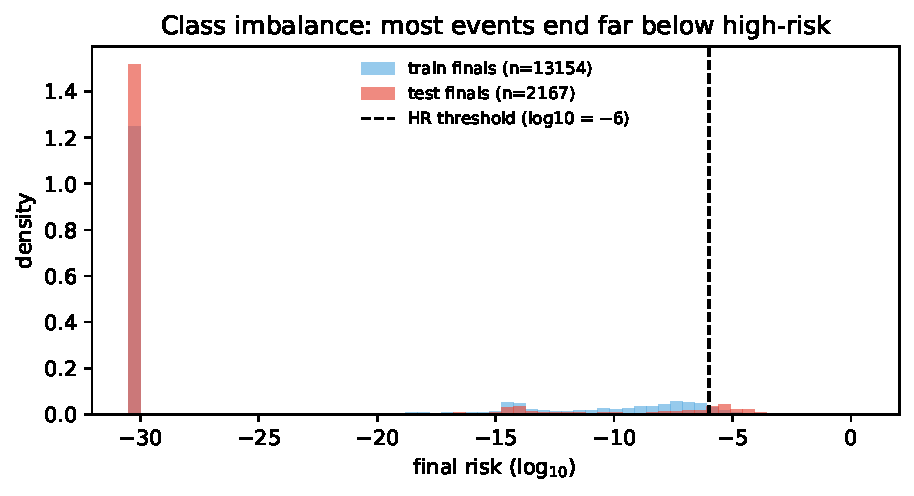
\includegraphics[width=0.92\linewidth]{figures/fig_risk_distribution.pdf}
  \caption{Density of final log\(_{10}\) risk for train-event finals and official test finals. Dashed line: HR threshold \(r=-6\). Source: Zenodo DOI~\texttt{10.5281/zenodo.4463683}.}
  \label{fig:eda}
\end{figure}

\begin{figure}[htbp]
  \centering
  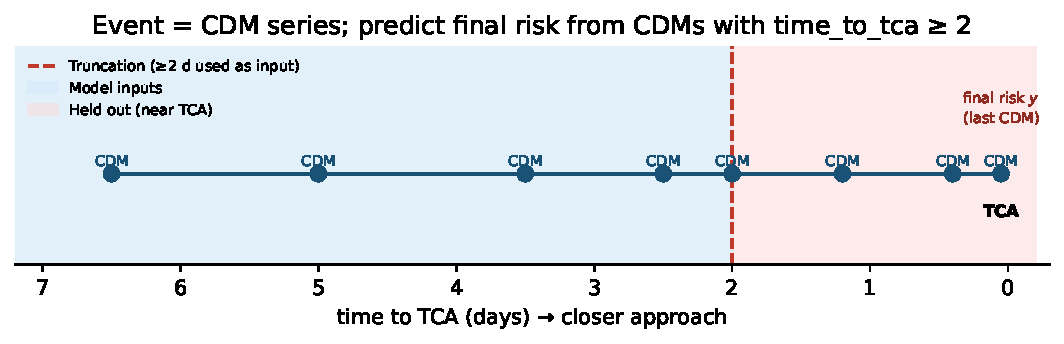
\includegraphics[width=0.92\linewidth]{figures/fig_cdm_timeline.pdf}
  \caption{Schematic event: CDM series vs time-to-TCA. Inputs use only messages with time-to-TCA \(\ge 2\) days; target is final risk near TCA~\citep{kelvins2019challenge,uriot2021collision}.}
  \label{fig:timeline}
\end{figure}

\section{Preliminary Methodology and Results}

\textbf{Evaluation.}
Scores use official Zenodo test events (\(n=2167\)). Inputs: public CDMs with time-to-TCA \(\ge 2\). Metrics: \(F_2\) (HR vs non-HR), \(\mathrm{MSE}_{\mathrm{HR}}\) on true HR with risk clipped at \(-6.001\), and \(L=\mathrm{MSE}_{\mathrm{HR}}/F_2\)~\citep{uriot2021collision}. The test set is used here only to reproduce published baselines, not to select models.

\textbf{Baselines.}
CRP predicts \(\hat r=-5\) always. LRP copies the latest eligible early risk (minimum time-to-TCA among CDMs with time-to-TCA \(\ge 2\)). Table~\ref{tab:preliminary-results} and Figure~\ref{fig:baselines}: CRP is weak (\(L\approx 2.50\)); LRP is strong (\(L\approx 0.694\), \(F_2\approx 0.739\), \(\mathrm{MSE}_{\mathrm{HR}}\approx 0.513\)), matching Uriot et~al.\ within rounding~\citep{uriot2021collision}. Later models must beat or explain LRP under rare-event metrics.

\begin{table}[htbp]
  \centering
  \caption{Preliminary baselines on the official Zenodo test set (\(n=2167\); 150~HR). \(F_2\) higher is better; \(\mathrm{MSE}_{\mathrm{HR}}\) and \(L\) lower are better.}
  \label{tab:preliminary-results}
  \begin{tabularx}{0.95\linewidth}{@{}Xcccc@{}}
    \toprule
    Model & Split & \(F_2\) & \(\mathrm{MSE}_{\mathrm{HR}}\) & \(L\) \\
    \midrule
    CRP (\(\hat r=-5\)) & Official test & 0.271 & 0.679 & 2.504 \\
    LRP (latest early risk) & Official test & 0.739 & 0.513 & 0.694 \\
    \bottomrule
  \end{tabularx}
\end{table}

\begin{figure}[htbp]
  \centering
  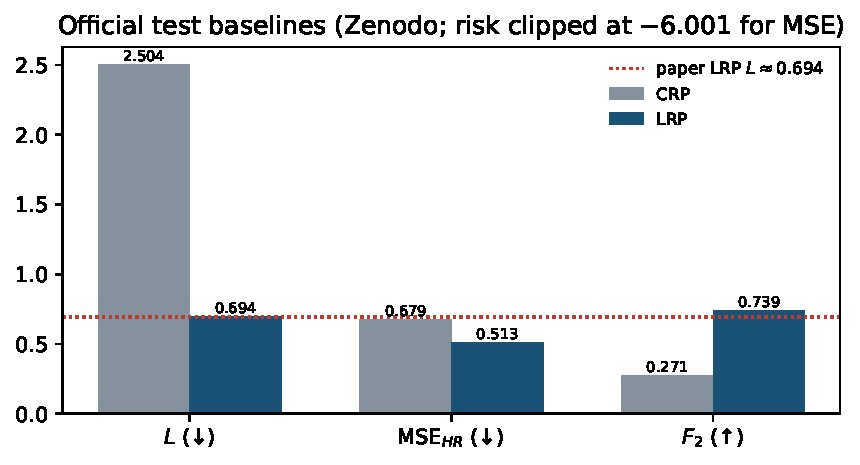
\includegraphics[width=0.88\linewidth]{figures/fig_baseline_metrics.pdf}
  \caption{Official-test CRP vs LRP. Dotted line: published LRP loss \(L\approx 0.694\)~\citep{uriot2021collision}.}
  \label{fig:baselines}
\end{figure}

\textbf{Planned methods.}
Much signal sits in the last early risk; residual value is in LRP failures (including jumps) and calibrated probabilities. Path: course models (linear/logistic, tree ensembles, later PyTorch nets) under one event-level protocol, then a two-stage calibrated \(P(\mathrm{HR})\) + magnitude head with reliability diagrams and a failure atlas. We will selectively trial out-of-syllabus ideas (temporal encodings, isotonic/temperature scaling, abstention) when they address jump uncertainty---cited as prior art when related to competition winners, never as ``re-run Kelvins to win''~\citep{uriot2021collision}.

\section{Next Steps, Reproducibility, and Ownership}

\textbf{Next steps.}
(1)~Freeze metrics; deepen EDA (missions, jump candidates).
(2)~Features (latest CDM, deltas, aggregates) + course models vs LRP.
(3)~Two-stage model + calibration + failure atlas; optional ambitious ablations.
(4)~Fair PyTorch / sequence ablation if justified by jump analysis.
(5)~Report polish and oral defence.

\textbf{Risk/contingency.}
LRP may remain hard to beat and train/test mismatch may destabilise rankings~\citep{uriot2021collision}. Contingency: report course models fairly; emphasise calibration and failures even if gains over LRP are small---that outcome still answers the RQs.

\textbf{Reproducibility.}
Public GitHub with meaningful history; seeds and environment pinned when stochastic methods appear; Zenodo DOI for data; scripts regenerate tables/figures. Large raw files are not committed.

\section*{Declaration of Contributions and AI Use}

Teamwork: We jointly chose the ESA early-risk problem, fixed the RQs and evaluation protocol, and reviewed this proposal before submission.

Individual contributions:
Pedro Jon Fuentes Garc\'es: problem framing, research questions, domain narrative, figure captions, and proposal drafting.
Mario Fern\'andez Velasco: data handling, CRP/LRP baseline reproduction, metrics, tables, and figure generation from code.
Both: protocol decisions and final approval.

AI tools: Cursor (AI assistant) helped with literature organisation, Zenodo download, baseline metric code, figure generation from that code, and a structural draft of this text, which we edited and own. Each member can defend the protocol, CRP/LRP numbers, and two-stage plan. Verification: recomputed official-test CRP/LRP with \(L_{\mathrm{LRP}}\approx 0.694\) vs Uriot et~al.~\citep{uriot2021collision}. AI is not an author.

\BAMprintbibliography

\end{document}
